Le contenu des mini-jeux est très varié : jeu de rôle, jeu de gestion, jeu de plateforme, etc.
L'analyse des différences et des ressemblances entre ceux-ci, afin de définir ensuite une grammaire de description de jeux, est d'autant plus complexe.

Les difficultés d'implémentation des mini-jeux sont elles aussi différentes.
8 exemples concrets de jeux sont développés par la suite.
Cela permet d'appuyer l'analyse de ce que contient un mini-jeu.

Ces jeux n'ont pas été choisi par hasard : chacun possède un intérêt dans la description de ses règles et son implémentation.

\vspace{0.5cm}

\begin{tabular}{l|l}
 Jeu & Intérêt majeur \\
 \hline
 Pacman & ?? \\
 1942 & Vagues d'ennemis \\
 Volley & Logique de score \\
 Course & Intelligence artificielle \\
 Mario & Niveaux \\
 Game\&Watch & ?? \\
 Billard & Collisions \\
 Jeu de Gestion & Ressources \\
\end{tabular}

\vspace{0.5cm}

Tout d'abord, chaque jeu est présenté succintement, illustré par une capture d'écran d'une implémentation effectuée.
Dans un second temps, une analyse de leur contenu sera effectuée, appuyée par un tableau comparatif et les diagrammes UML de ces jeux.

\subsection{Présentation des mini-jeux}

\note{c'est pour l'instant un bête copier coller de chacun, les fautes n'ont pas été corrigés.
On retravaillera cette sous-partie pour homogénéiser les différentes descriptions}

\subsubsection{Pacman}


\begin{minipage}{9cm}
Ce jeu est une adaptation du jeu classique de Pacman. 
Le joueur contrôle le TUX via les touches du clavier. 
Son but est de manger toutes les pommes sur le terrain tout en évitant les Microsoft qui essayent de l’attraper. 
Pour arriver à cet objectif, le joueur dispose de 3 vies. Le TUX peut manger des pommes en or pour pouvoir détruire les Microsoft pendant
une courte durée et marquer des points supplémentaires. Concernant l’affichage, le joueur voit le nombre de vies restantes, 
son score ainsi que le temps durant lequel les Microsoft restent vulnérables. Le jeu est adaptable car il est facile d’initialiser 
la carte à partir d’images et d’un fichier Json.
\end{minipage}
\hfill
\begin{minipage}{6cm}
 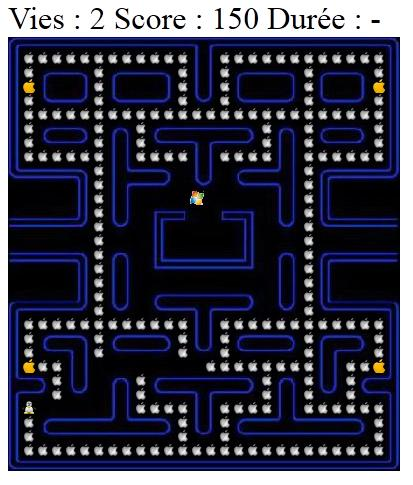
\includegraphics[width=\linewidth]{img/capturejeu_pacman}
\end{minipage}


\subsubsection{1942}

\begin{minipage}{6cm}
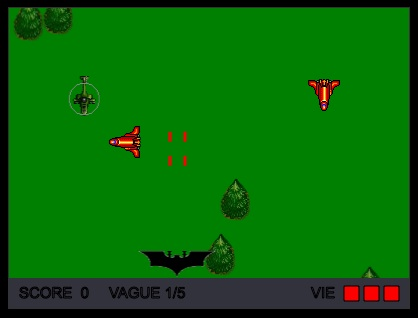
\includegraphics[width=\linewidth]{img/capturejeu_1942}
\end{minipage}
\hfill
\begin{minipage}{9cm}
Dans ce shoot them up (jeu d’action où le joueur fait face à une multitude d’ennemis), 
le joueur contrôle un vaisseau armé de deux canons pour détruire tous les véhicules adverses et gagner ainsi des points. 
Le joueur possède 3 vies pour faire le maximum de points. Lorsque le joueur perd une vie, il devient invincible durant une courte durée 
pour reprendre la main. Le vaisseau est contrôlé via le clavier. En ce qui concerne les ennemis, 
ils suivent des déplacements prédéfinis qui peuvent être paramétrés. 
Le joueur n’est pas obligé de tuer tous les ennemis mais le but est quand même de faire le plus grand score.
\end{minipage}

\subsubsection{Volley}

\begin{minipage}{9cm}
CowCow volley party est un mini jeu humoristique mettant en scène deux vaches jouant au volley.
On peut jouer à ce jeu en mode solo contre une IA ou à deux joueurs. 
Le but est de remporter 2 sets, sachant que remporter un set revient à marquer \note{xxx} points. 
La vache dispose de 3 coups différents : passe courte, passe longue et un smash.
Les règles de ce jeu sont les mêmes que celles du volley classique.
La vache est contrôlée au clavier aussi bien en mode multijoueur qu’en mode solo.
\end{minipage}
\hfill
\begin{minipage}{6cm}
 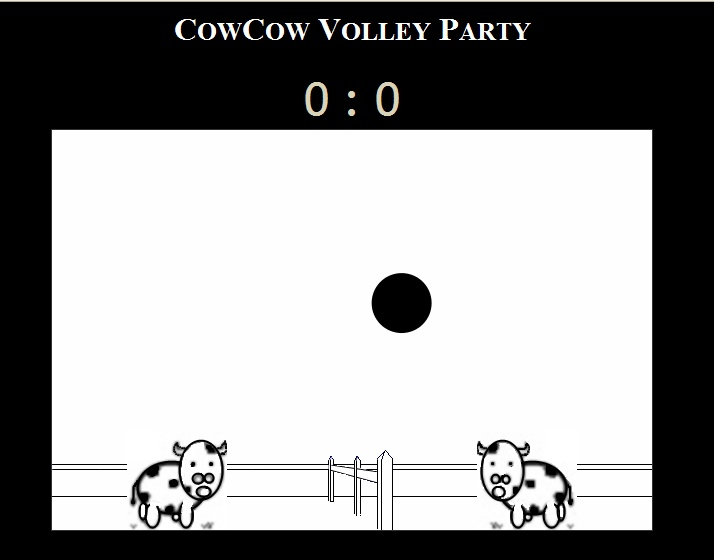
\includegraphics[width=\linewidth]{img/capturejeu_volleycowcow}
\end{minipage}


\subsubsection{Course}

\begin{minipage}{6cm}
 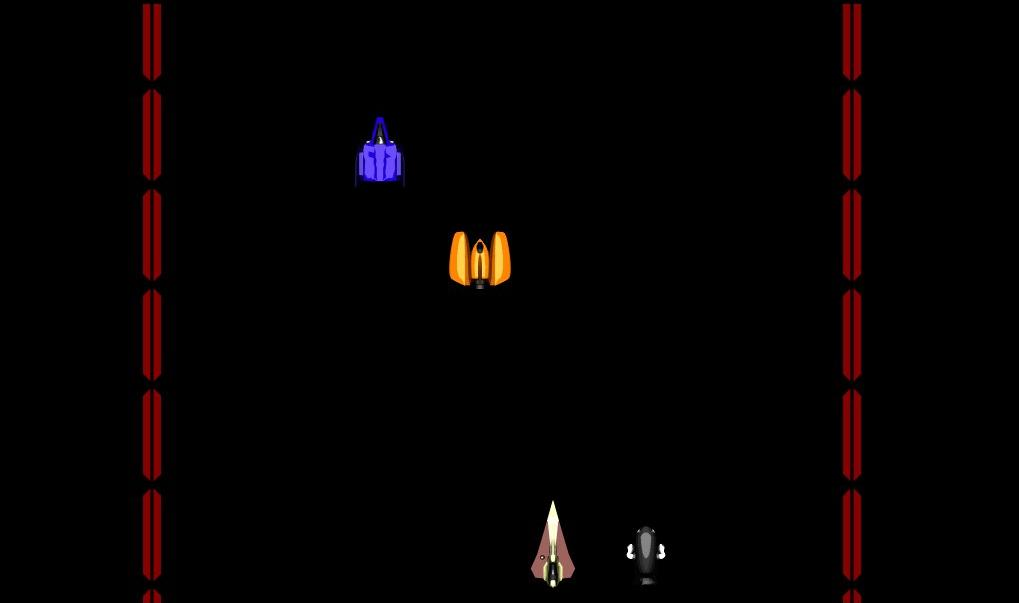
\includegraphics[width=\linewidth]{img/capturejeu_course}
\end{minipage}
\hfill
\begin{minipage}{9cm}
Ce jeu de course futuriste pour le web permet au joueur de se frotter à des intelligences artificielles pour faire le meilleur temps. 
Ce  n’est pas un jeu de course classique : en effet des bonus se trouvent sur le circuit :
un turbo, un bonus permettant d’augmenter le temps d’un des autres joueurs, un autre changeant la position d'un adversaire, etc. 
De plus, il existe différentes zones de circuit ayant des effets divers : inversion des commandes, changement de vitesses, etc.
Le joueur peut choisir son véhicule parmi une sélection de 12 vaisseaux différents. 
Le contrôle se fait au clavier. Ce jeu est adaptable : en effet, il est possible de créer facilement des circuits ainsi que des nouveaux bonus. 
Il serait aussi possible de mettre en place un système de lecture de fichier pour configurer les paramètres des différentes courses.
\end{minipage}

\subsubsection{Mario}

\begin{minipage}{9cm}
Ce mini-jeu de plateforme reprend le principe des jeux du style de mario bros.
Un personnage, contrôlé au clavier et représenté par un rectangle, peut se déplacer sur les côtés ou sauter.
Il doit avancer au maximum, sans être touché par des ennemis, dessinés par des triangles, et sans tomber dans les trous du terrain.
Le personnage peut faire perdre des points de vie aux ennemis jusqu'à les tuer en leur sautant dessus. 
S'il les touche sur les côtés, il meurt et la partie est terminée.
La caméra avance lorsque le joueur avance suffisamment. Le joueur peut revenir à gauche jusqu'à la limite de l'écran.
Le terrain est généré aléatoirement et est infini.
Le but du jeu est d'obtenir le plus grand score. Le score diminue avec le temps et augmente lorsqu'un ennemi est tué ou que le personnage avance.
\end{minipage}
\hfill
\begin{minipage}{6cm}
 \framebox[\linewidth]{\parbox{\linewidth}{~ \vspace{4cm} Capture à venir ~\\~\\}}
\end{minipage}


\subsubsection{Game \& Watch}

\begin{minipage}{6cm}
 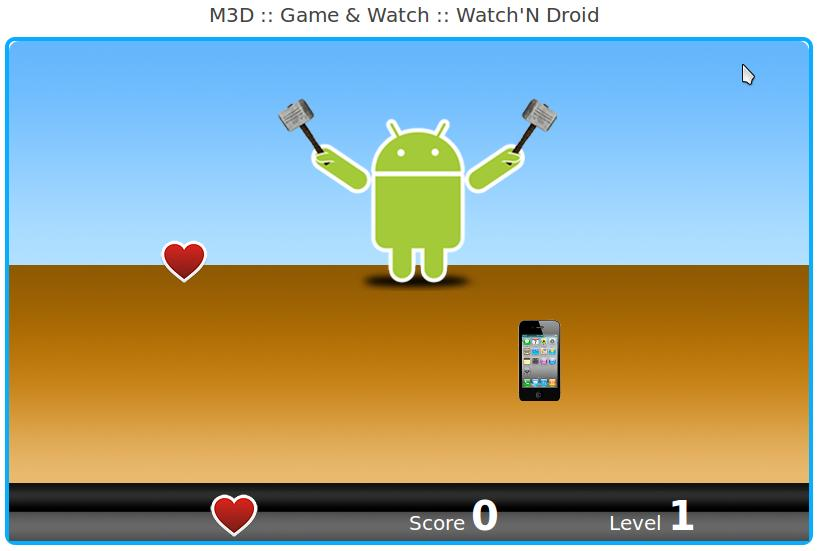
\includegraphics[width=\linewidth]{img/capturejeu_watchndroid}
\end{minipage}
\hfill
\begin{minipage}{9cm}
Watch’N’Droid est un mini-jeu du style Game \& Watch. 
Le joueur doit chasser ses ennemis avant que ces derniers ne l’atteignent. 
Les ennemis apparaissent un par un en bas de l’écran et montent pour atteindre le joueur à une certaine vitesse.
Cette dernière varie en fonction du niveau dans lequel le joueur se trouve. 
L’utilisateur est armé de deux marteaux pour détruire l’ennemi et donc marquer des points. 
Lorsque l’ennemi atteint le joueur se dernier perd une vie.
Lorsqu’il ne lui reste que deux vies, des vies bonus apparaissent sur l’écran et le joueur peut les ramasser. 
Lorsque le nombre de vie arrive à zéro, le joueur a la possibilité d’enregistrer son score si ce dernier fait partie
 des cinq meilleurs scores qui sont actuellement enregistrés.
\end{minipage}

\subsubsection{Billard}

\begin{minipage}{9cm}
Ce mini-jeu de billard est un jeu multijoueurs au tour par tour. 
Il reprend les règles classiques du billard anglais (chaque joueur doit rentrer toutes les boules d’une couleur puis la noire). 
D’un point de vue gameplay, le joueur contrôle la queue qui pointe automatiquement vers la boule blanche via sa souris. 
Le joueur peut ainsi choisir l’angle avec lequel il compte frapper la boule blanche et en fonction du temps pendant lequel
 le joueur laisse le clic de la souris enfoncé, le tir est plus ou moins fort. 
Pour l’affichage, chaque joueur voit le nombre de boules rentrés ainsi que sa couleur. 
Une icône verte apparait au niveau du joueur qui doit jouer. 
Le cadre bleu en bas de l’écran affiche la personne ayant gagné la partie !
\end{minipage}
\hfill
\begin{minipage}{6cm}
 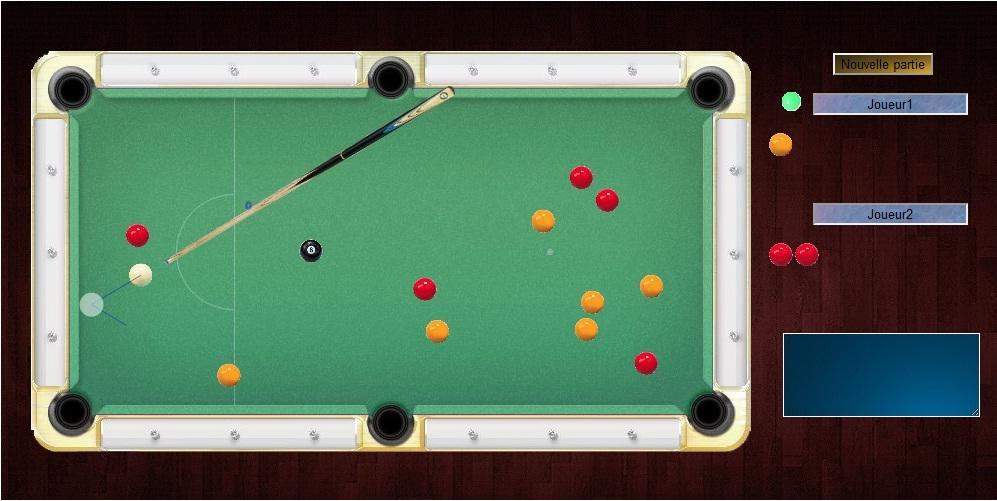
\includegraphics[width=\linewidth]{img/capturejeu_billard}
\end{minipage}


\subsubsection{Gestion}

\begin{minipage}{6cm}
 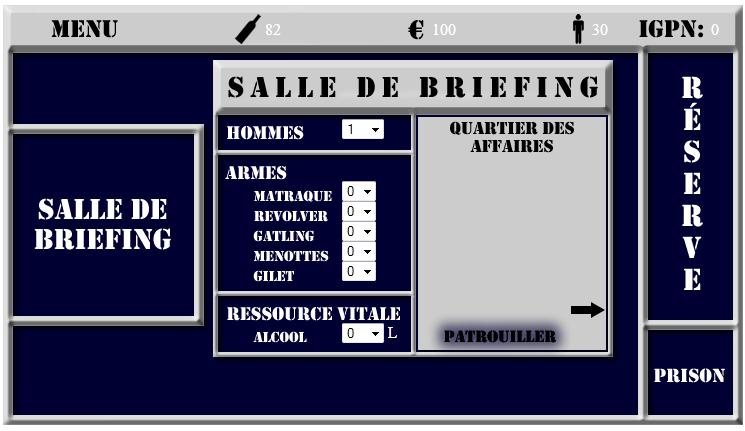
\includegraphics[width=\linewidth]{img/capturejeu_gestion2}
\end{minipage}
\hfill
\begin{minipage}{9cm}
Le jeu commissariat est un jeu de gestion du style Farmville. 
Le but est de maintenir et améliorer le commissariat en fonction des ressources disponibles.
Les ressources sont au nombre de quatre : le nombre de policiers, l’argent, l’indice IGPN et l’alcool. 
Il y a trois actions disponibles pour le joueur. Il peut envoyer des policiers en mission dans un quartier 
choisi pour ramener de l’argent ainsi qu’un prisonnier. Si un prisonnier est ramené, le joueur a la possibilité 
de libérer le prisonnier contre de l’argent ou de le tabasser (avec un fort risque de pénalité). 
Il peut aussi acheter des équipements ainsi que de l’alcool avec son argent. L’alcool est une ressource qui diminue constamment, 
le joueur doit veiller à toujours en avoir pour ne pas perdre. Il peut aussi perdre avec un indice d’IGPN trop élevé, cet indice 
monte avec toutes les mauvaises actions (tabasser un prisonnier, etc.).
\end{minipage}

\subsection{Analyse des mini-jeux}

Suite au développement de ces mini-jeux, nous avons voulu analyser le contenu de ces différents jeux.
Pour cela, le tableau suivant récapitule différents aspects des jeux.

\note{inclure le tableau de google docs, en renvoyant peut être les colonnes pour mieux l'adapter à ce qu'on a fait dans la grammaire}

\vspace{0.5cm}

\begin{tabular}{|l|l}
\hline
 Jeu &   \\
\hline
 Pacman &  \\
\hline
 1942 &   \\
\hline
 Volley &  \\
\hline
 Course &  \\
\hline
 Mario &  \\
\hline
 Game\&Watch & \\
\hline
 Billard &  \\
\hline
 Jeu de Gestion & \\
\hline
\end{tabular}

\vspace{0.5cm}

Ce tableau permet de mieux identifier les différences et points communs entre les différents jeux.

On y voit par exemple que les objectifs au cours d'un niveau (ou pour un jeu sans niveau) revient souvent à atteindre une certaine zone
appelée ligne d'arrivée, ou éventuellement remplir des conditions de temps ou de ressources. En effet, à la fois la vie et le score
peuvent être vus comme une ressource : il s'agit d'un état, et une condition sur celui-ci est nécessaire à la victoire.
En faisant des conjonctions et des disjonctions de ces différentes possiblités, il est possible de définir 
les conditions de victoire pour tous les jeux (sauf le jeu de gestion).

En revanche, si on regarde comment le monde est construit, il est très différent d'un jeu à l'autre.
Pour certains comme Pacman, il est défini par une grille, pour d'autres comme le jeu de course, il est défini via un anneau.

Le tableau nous permet de voir assez clairement que le jeu de gestion est très différent des autres jeux.
Nous avons donc décidé de ne pas prendre en compte ce type de jeux.
Nous allons donc essayé de tirer des points communs entre les autres jeux, pour définir des concepts qui seront détaillés dans 
les parties suivantes.
Retirer de notre grammaire les jeux de gestion n'empêchent pas de couvrir un nombre important de jeux.
Il serait possible par exemple de définir plusieurs grammaires, chacune couvrant une catégorie de jeux afin de pouvoir
créer plusieurs types de jeux. Ainsi on pourrait créer une autre grammaire spécialement pour les jeux de gestion.
De la même façon, il est difficile de trouver des points communs entre les 7 mini-jeux restants, et un jeu de rôle où par exemple le joueur
doit réaliser plusieurs quetes.
Cependant, nous nous sommes concentrés pour le moment sur une unique grammaire décrivrant les 7 mini-jeux.

\note{Lister les concepts trouvés}
